\section{Materials and Methods}
\subsection{Materials}\label{Materials}
\begin{itemize}
	\item Armadillo IV with Vibro crop implement
	\item Turnigy 130A Watt Meter and Power Analyzer
	\item Camera
\end{itemize}
\subsection{Test description}
The test aims to provide an estimate of the power consumption during normal use of the Armadillo IV while using the Vibro crop implement. The depth of the cultivator is adjusted to 1.5 cm relative to the front wheels, see figure \ref{fig:vibro_crop_working_depth}.
\begin{figure}[hbtp]
	\centering
	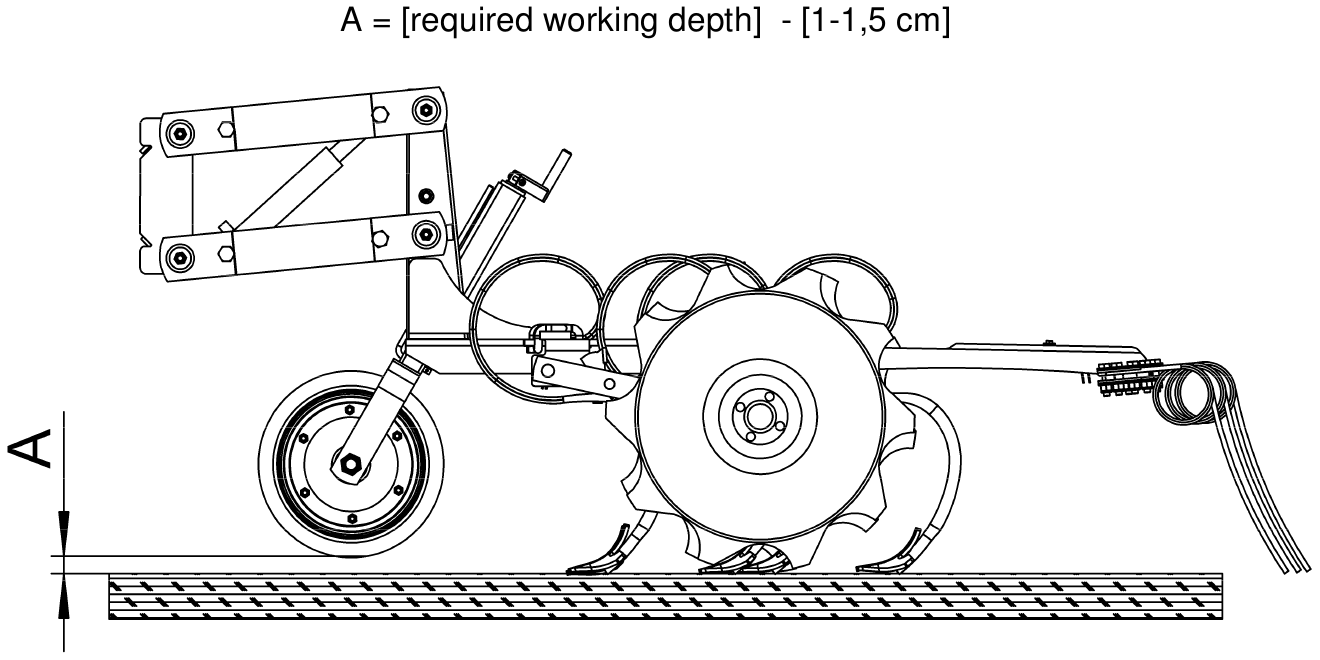
\includegraphics[width=0.7\linewidth]{vibro_crop_working_depth}
	\caption{Working depth of cultivator during normal use \cite{vibro_crop}}
	\label{fig:vibro_crop_working_depth}
\end{figure}
Due to the fact that the front wheels also dig into the ground, the working depth is around 2-3 cm \cite{vibro_crop}. The Armadillo IV is driven a distance of 10 m 5 times with varying speeds for each 10 m run. The power consumption is measured during each run, using the Turnigy watt meter and an external camera filming the watt meter.
The motor controllers provide a way of measuring the power consumption as well. This data can be accessed through ROS bags. The tests will also be used to see if the internal power measuring will produce results similar to the Turnigy watt meter. The watt meter is connected between the battery of the right side of the Armadillo IV as seen in figure \ref{fig:wattMeter}.

\begin{figure}[hbtp]
	\centering
	
\includegraphics[width=0.7\linewidth]{wattMeter}
	\caption{Watt meter connection}
	\label{fig:wattMeter}
\end{figure}

It was decided to do the 5 runs on the same piece of field due to the condition of the field. Corn had previously been sown on the field and had not been maintained and therefore contained high amounts of grass which would be caught by the cultivator, see figure \ref{fig:grassProblem}.
The grass was removed and the piece of field was run through 4 times before the actual test. 
\begin{figure}
\centering
	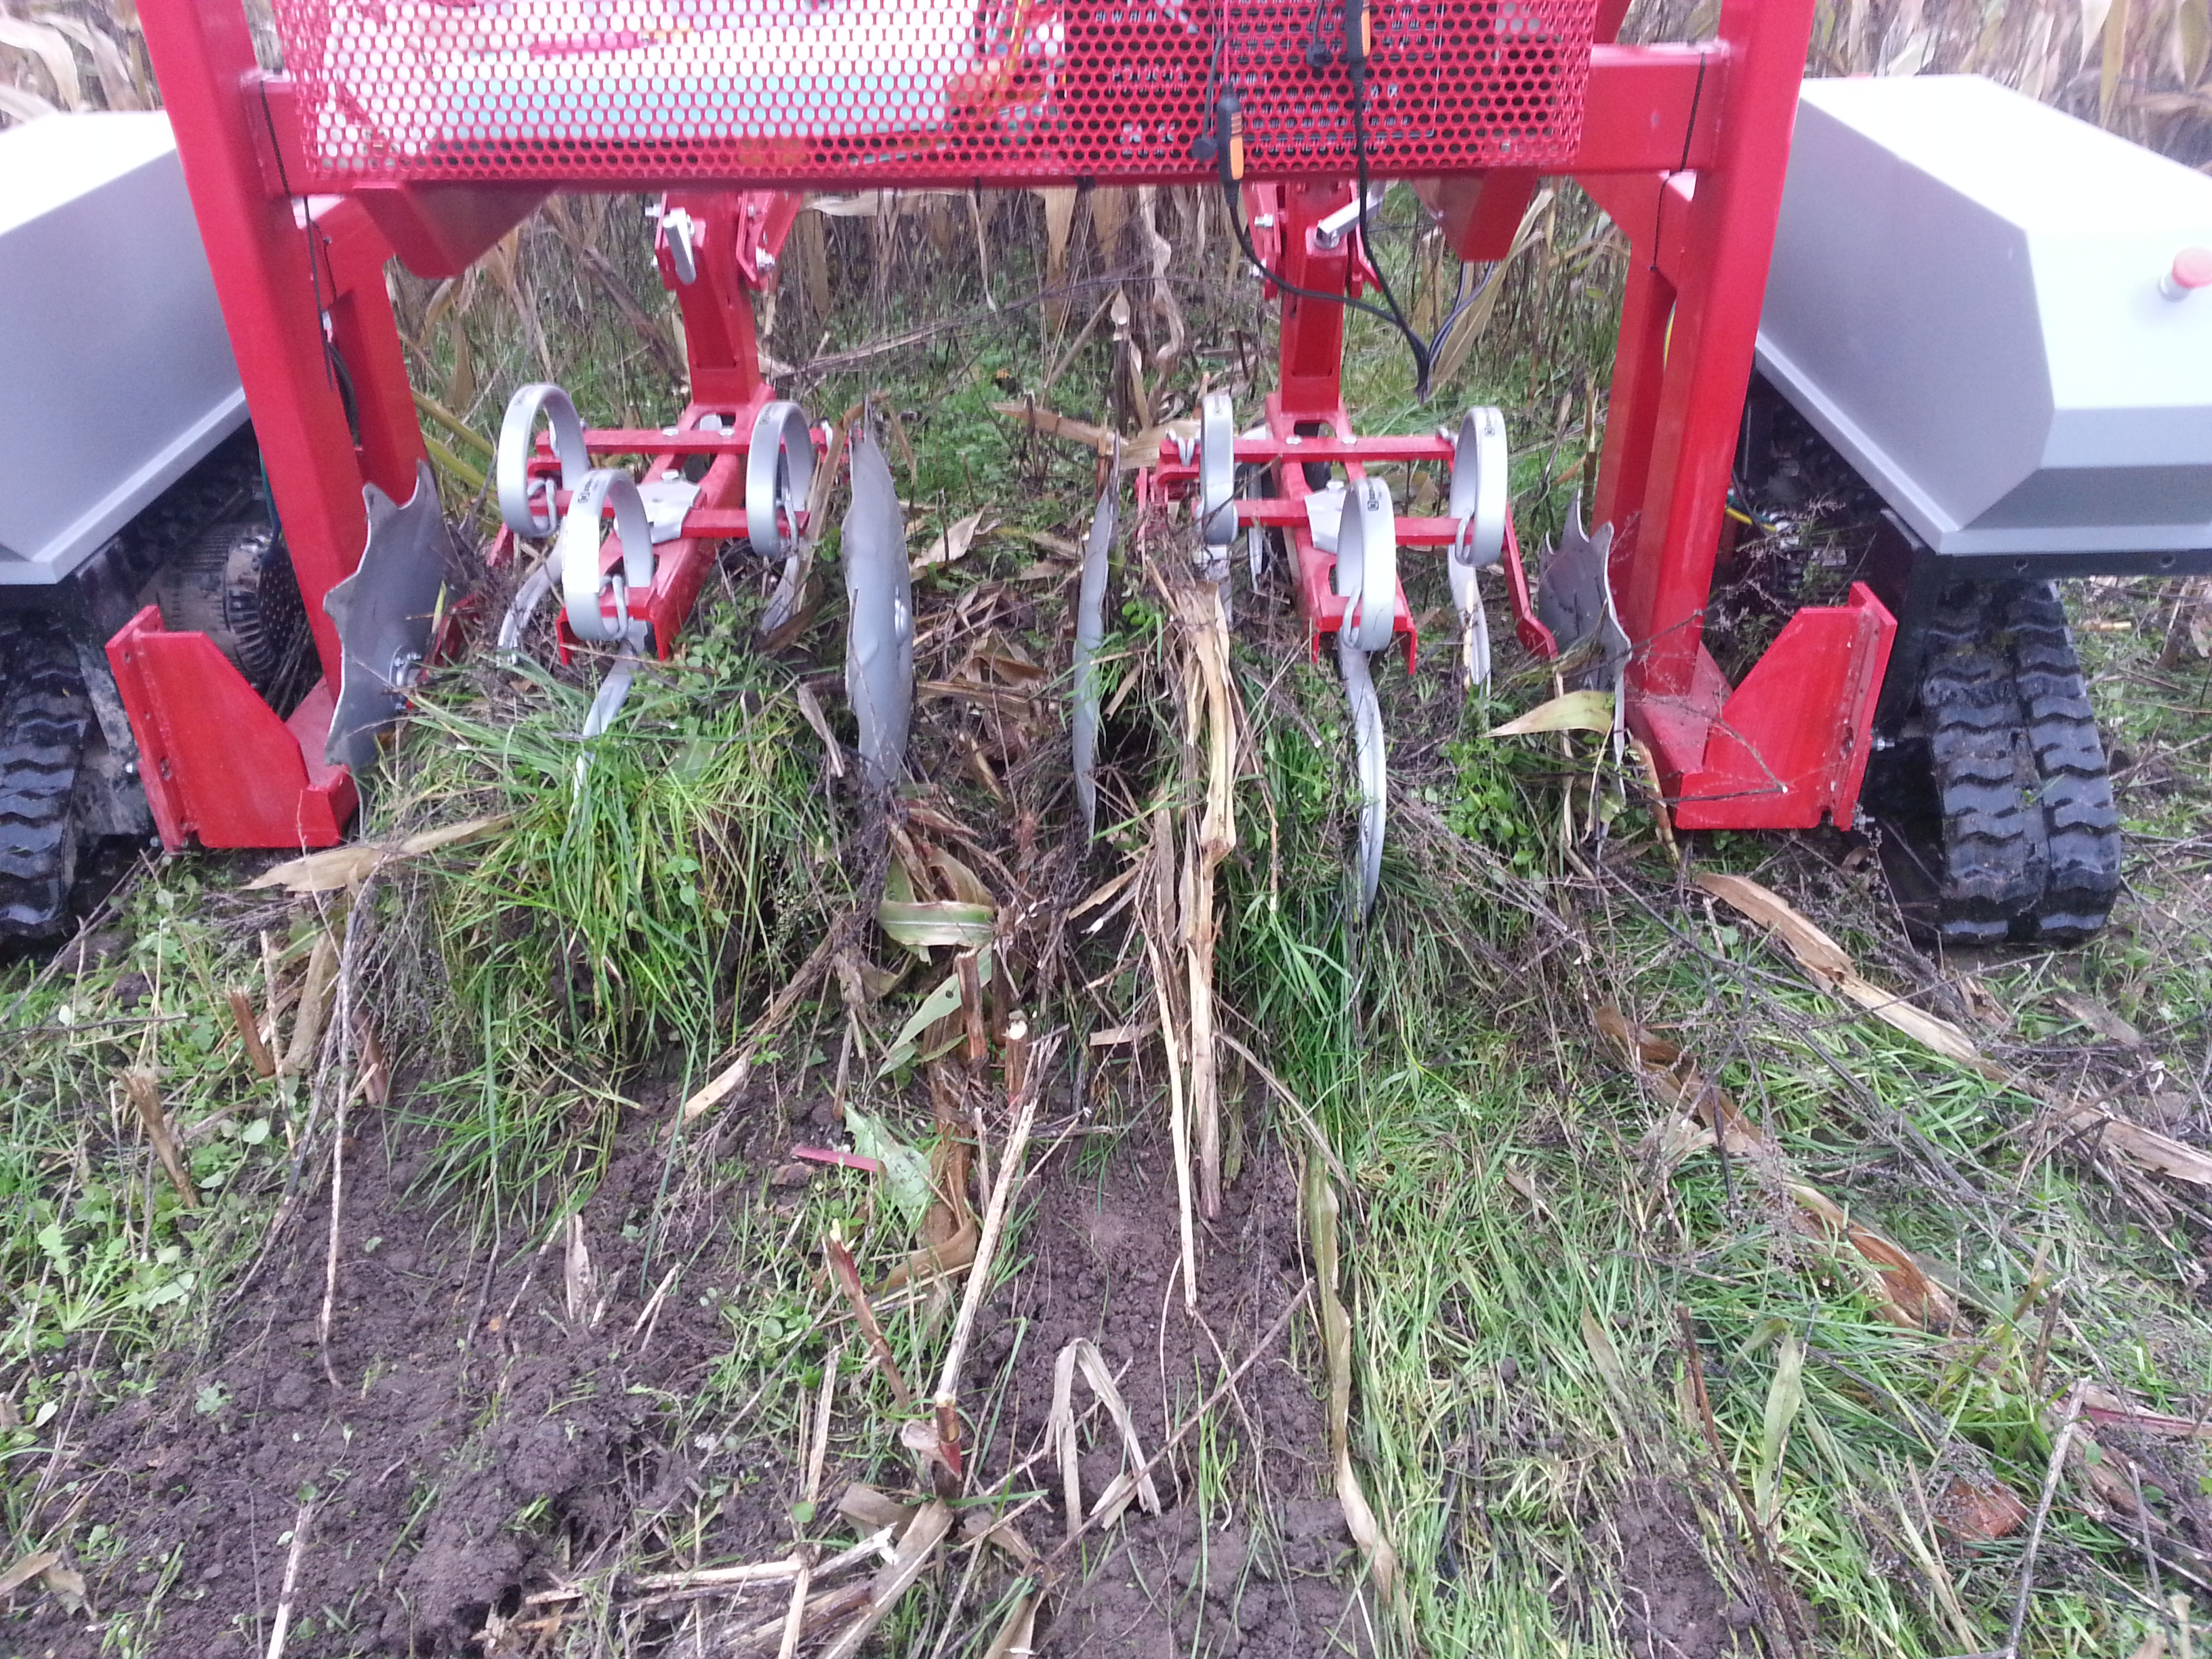
\includegraphics[trim = 2cm 15cm 10cm 5cm, clip ,width=0.6\linewidth]{grassProblem}
	\caption{Grass caught by the cultivator during a run.}
\label{fig:grassProblem}
\end{figure}


